%! Author = joels
%! Date = 27/01/2022

\section{Typ Polymorphismus}
\subsection{Vererbung}
\textbf{$\rightarrow$ Zur Einfachheit nur Single Inheritance}\\
\textbf{Sonst:} Diamond Problem (Wenn in oberster Klasse Instanzvariablen vorhanden wären)\\
\textbf{Zwei Aspekte:}
\begin{itemize}[topsep=0pt]
    \itemsep -0.2em
    \item Code Reuse: Subklasse erbt variablen \& Methoden der Basisklasse
    \item Typ-Polimorphismus: Objekt der Subklasse ist auch vom Typ der Basisklasse
    \SubItem{Dynamischer Typ: Zur laufzeit, Statischer Typ: Deklarierter $\rightarrow$ Compiler}
\end{itemize}
\textbf{Type Test \& Cast:} Entscheiden mit Descriptor $\rightarrow$ Vererbungshierarchie so lange traversieren, bis es keine Basisklasse mehr gibt, oder man den Typ gefunden hat.\\

\subsection{Ancestor Tables}
\begin{minipage}{0.5\linewidth}
    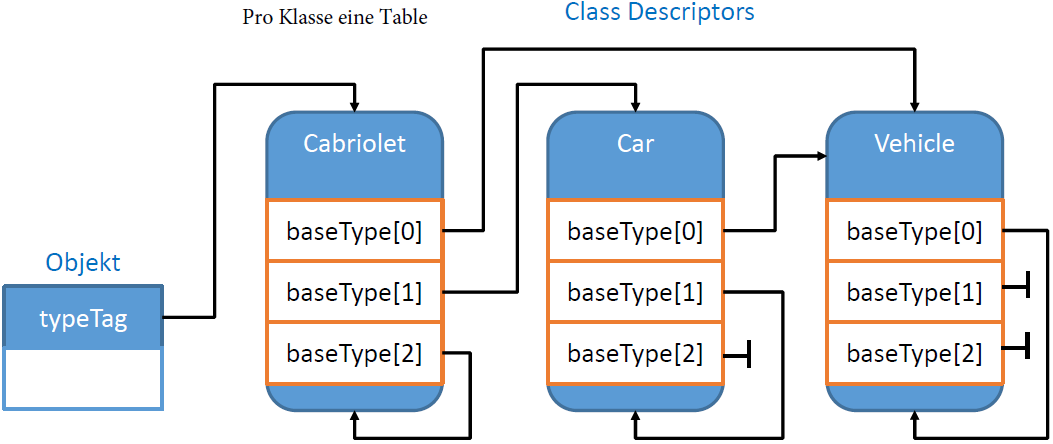
\includegraphics[width=\linewidth]{ancestor_table}
\end{minipage}
\begin{minipage}{0.5\linewidth}
    \begin{itemize}
        \item Konstante Zeit für Type Tests \& Casts
        \SubItem{Alternative: Dynamische Tabelle mit Längenprüfung}
        \item Anzahl Stufen kann begrenzt sein
        \item Funktioniert nur bei Single-Inheritance
    \end{itemize}
\end{minipage}

\subsection{Casts}
\begin{lstlisting}
// instanceof
var instance = checkPointer(pop());
var target = checkClassDescriptor(instruction.Operand);
var desc = heap.getDescriptor(instance);
var level = target.getAncestorLevel();
var table = desc.getAncestorTable();
push(table[level] == target);
// Zusätzlich prüfen:
// - Wenn instance null ist: False
// - Dynamische Länge der table --> Level könnte grösser sein als table.length

// checkcast
if (!checkBoolean(pop())) {
    throw new VMException("Invalid cast");
}
push(instance)
// Unterschied zu instanceof:
// - null kann man immer casten !!
// Im null-Fall beachten:
// null in instanceof T --> False
// (T)null --> succeeds
\end{lstlisting}

\subsection{Virtuelle Methoden}
Instanzmethoden können überschrieben werden. $\rightarrow$ Bei virtuellen Methodenaufruf entscheidet der dynamische Typ.\\
\begin{minipage}{0.4\linewidth}
    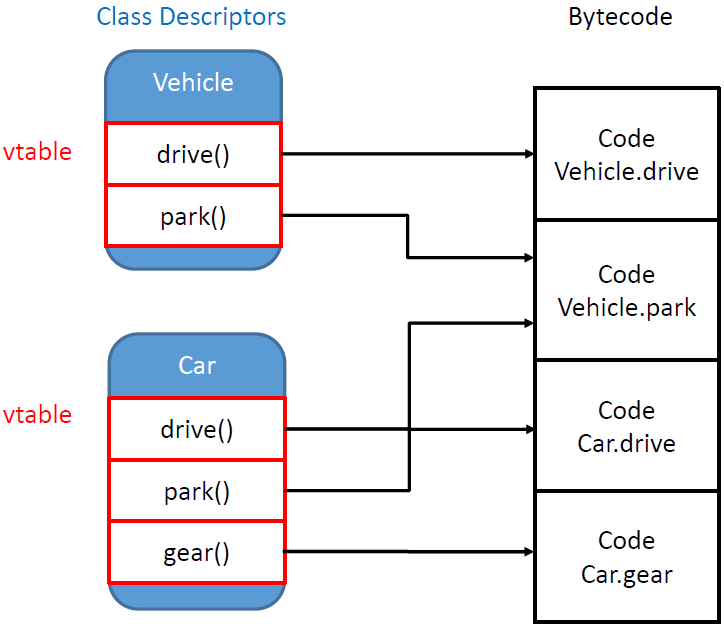
\includegraphics[width=\linewidth]{vtable}
\end{minipage}
\begin{minipage}{0.6\linewidth}
    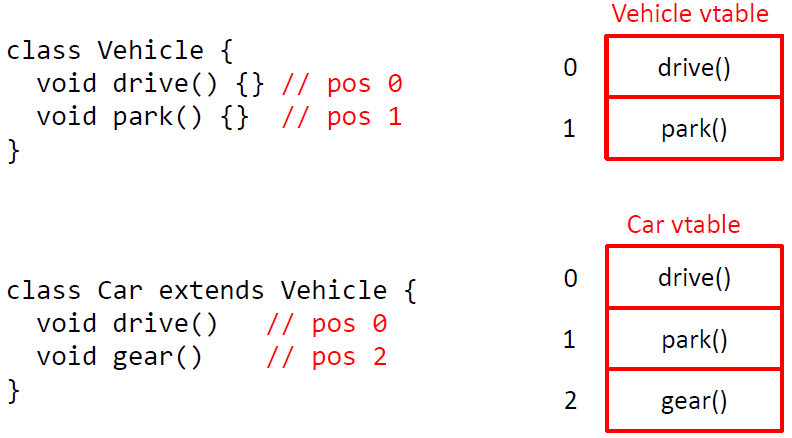
\includegraphics[width=\linewidth]{vtable_methods}
\end{minipage}
\begin{itemize}[topsep=0pt]
    \itemsep -0.2em
    \item Methoden von Basisklasse oben, eigene unten
    \item Position von jeder Methode ist statisch bekannt im deklariertem Typ
    \item Funktioniert nur bei Single Inheritance
    \item Loader präpariert die vtable und position
\end{itemize}
\begin{lstlisting}
// invokevirtual
// pop arguments
var staticMethod = checkMethodDescriptor(instruction.Operand);
var target = checkPointer(pop());
var desc = heap.getDescriptor(target);
int pos = staticMethod.getPosition();
var vtable = desc.getVirtualTable();
var dynamicMethod = vtable[pos];
// call dynamic method
\end{lstlisting}

\subsection{Interfaces}
\begin{itemize}[topsep=0pt]
    \itemsep -0.2em
    \item Interfaces global durchnummerieren
    \item Pro Class decriptor eine Interface Table (itable)
    \item Einträge in itable verweisen auf vtable
    \item Class Descriptor verweist auf itable (ibase-Pointer)
\end{itemize}